\documentclass{article}

% Language setting
% Replace `english' with e.g. `spanish' to change the document language


% Set page size and margins
% Replace `letterpaper' with `a4paper' for UK/EU standard size
\usepackage{geometry}
 \geometry{
 a4paper,
 total={170mm,257mm},
 left=20mm,
 top=20mm,
 }
%Packages
%Coloums

%\usepackage{tabularx}
%\usepackage{amsmath}
\usepackage{graphicx}
\usepackage[colorlinks=true, allcolors=blue]{hyperref}
\usepackage{titlesec}
\usepackage[square,numbers]{natbib}

\graphicspath{ {./images/} }

\title{Project Life Cycles}
\author{Chris Hadden}
\bibliographystyle{abbrvnat}
\begin{document}

\maketitle

\tableofcontents

\section{(P1) The different phases in a project life cycle}
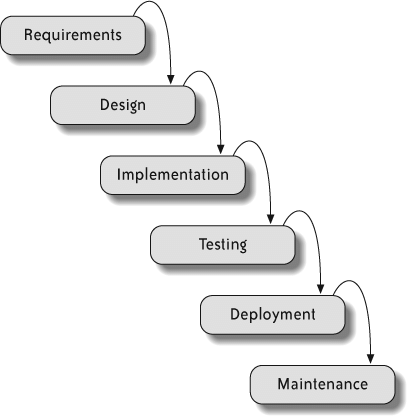
\includegraphics[scale=0.5]{Modern-Waterfall-Diagram}
\cite{modernwaterfall}
\subsection{Initiation phase}
The initiation phase is where we setup and define what the project is gonna be and who should produce this project.It is also to question if this project is necessary and who is it for is it for the stakeholders or a client or is there a target audience.

This phase in the project is equivalent to in waterfall is: Requirements

\subsection{Planning phase}
The planning phase is when we set the outcomes and it will be the reference document used by the project manager. If you have failed to planned then you are planning to fail. \\

The four points we have to consider are: 
\begin{itemize}
    \item What exactly are going to do
    \item How are we going to do it
    \item When are we going to do it
    \item How will we know when we're done
\end{itemize}

This phase in the project is equivalent to in waterfall is: Design

\subsection{Execution phase}
The execution phase the team are going to develop the product. This phase begins with a inital meet with a the client, this will be met with an onset of status reports and update. 

What is done in the the execution phase are:
\begin{itemize}
    \item Develop team
    \item Execute project management plans
    \item Set up tracking systems
    \item Status meetings
    \item Update project schedule
\end{itemize}

This phase in the project is equivalent to in waterfall is: Implementation/Deployment

\subsection{Finishing phase}

Once a project is completed the team will have to close it. Project managers will hold a meeting after the project has officially ended to evaluate what made the project become so successfully or what where the pit falls that causes the project to fail.

There are still task for the project manager to do after the project has officially closed.The project manager will have to create a project punch, this will create a list of points that didn't get accomplished during the life time of the project and to work with the team to complete them. Create a final project report and final project budget. Finally, they will need to collect all project deliverables and  documents and store them in a single place.

This phase in the project is equivalent to in waterfall is: Maintenance

\break
\section{(D1) The importance of each development phase of the identified project life cycle}

\subsection{Initiation Phase}
The initiation phase is important as it bootstraps our abstract ideas into a meaningful goal. This stage will develop a model and define how the project will be made but to do this we need to determine the need for the project.




\subsection{Planning phase}
During the planing phase we to pay a lot of attention so that we all understand how this project will be made and what is need to it be done. One of the easy ways to getting goals in S.M.A.R.T. This method ensures that the goals have been thoroughly thought thought and it also provides a clear understand of what is to be done. \\

The Smart goal are
\begin{enumerate}
    \item Particular: To establish precise objectives,
    \item Measurable: Establish standards by which you may gauge an objective's success.
    \item Attainable: Determine the most crucial objectives and the necessary steps to fulfil them.
    \item Realistic: You must to be able and prepared to work towards a certain objective.
    \item Timely: Establish a deadline for completing the task.
\end{enumerate}


\subsection{Execution phase}
The execution phase is the part where the team release the product. The responsibilities of the project manager will expand, this means that you have to be able to establish an efficient workflow and carefully monitor the progress of your team. 

Another responsibility that the project manager will have during this phase as well, is to consistently maintain collaboration between the project stakeholders. We have to do this because if we didn't then their wouldn't be the improve efficiency and increased productivity that we want in the project.

\subsection{Finishing phase}

Once a project is complete, the team must formally close it. Project managers generally hold a post mortem meeting to evaluate successes and failures. Project close helps a team identify things that went well and areas for improvement.

Once the project is complete, PMs still have a few tasks to complete before it is officially closed. They will need to create a project punchlist of things that didn’t get accomplished during the project and work with team members to complete them. Perform a final project budget and prepare a final project report. Finally, they will need to collect all project deliverables and  documents and store them in a single place. 

When a project is finished, the group needs to end it. Project managers will convene a post mortem meeting to assess what factors contributed to the project's success or identify potential failure points.

Even after the project is formally concluded, the project manager still has tasks to do.The project manager will need to draft a project punch, which will compile a list of tasks that were left undone over the project's duration and assign the team members to do them.Compile the project's final budget and report.Lastly, they must gather and keep all project deliverables and documentation in one location.    

\break
\bibliography{bibliography}


\section{Sources}
\url{https://kissflow.com/project/five-phases-of-project-management/}

\end{document}
